\chapter{Design} \label{design}

\section{Design Specification}
What are our system specs?

\section{System Overview}
Block diagram of how stethoscope works
\begin{figure}[!htb]
	\centering
	\fbox{
		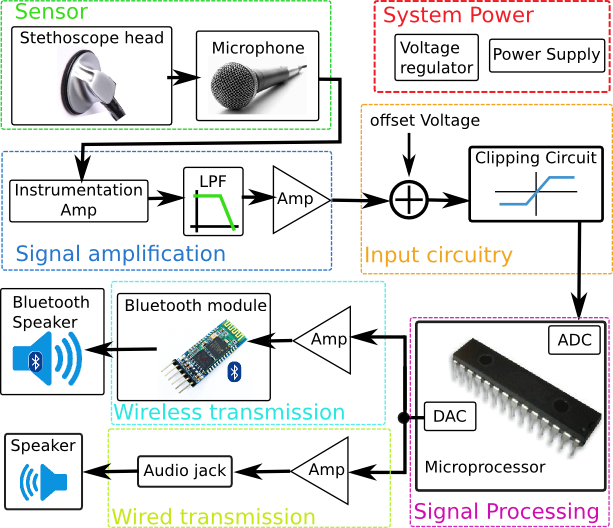
\includegraphics[resolution=120, width=375px, height=375px]{sys_overview.png}
	}
	\caption{System overview}
	\label{fig:sys_overview}
\end{figure}

\section{Maximum Sound Frequency}
In order to design our system we must determine what is the maximum sound frequency $f_{max}$ that it needs to measure. This frequency affects the design of the low pass filter and the sampling frequency needed for Analog to Digital Conversion. A lower $f_{max}$ results in a lower sampling frequency, which allows the microprocessor to carry out more computations per sample, and thus allows for higher order digital filters to be implemented. Higher order filters give greater flexibility in digitally manipulating the sound signal, and so would allow us to more accurately reproduce the sound characteristics of a conventional stethoscope.

An $f_{max}$ of 20kHz would work as this is the threshold of human hearing\cite[p.~163]{Stuart2011}, however it has been stated that the majority of heart and lung sounds occur at lower frequencies, within the range 37.5-1kHz\cite{Abella1992}. In order to determine $f_{max}$ 100 heart and lung sounds were analysed for their spectral content. Sound files were taken from an electronic resource used to train medical students in auscultation\cite{Coviello2014}, and three analyses were performed using MATLAB. 

The first analysis simply took a Fast Fourier Transform (FFT) of the sounds, summed the amplitudes and defined $f_{max}$ as the frequency at which this sum dropped below -80dB. In the second analysis all the sound signals were summed together, an FFT was performed on the resulting signal, and $f_{max}$ was defined to be the frequency at which the amplitude dropped below -80dB. In the third analysis the significant frequency components of each sound was calculated. Significant frequencies were defined as the range which contained 99.9\% of the signal energy. Signal energy was defined to be the sum of the squared FFT amplitudes and an iterative algorithm was used to calculate the range. The algorithm begins with a set that contains the signal's dominant frequency. It then adds to this set the next highest or lowest frequency, which ever has the larger FFT amplitude. The energy content of the set is compared with the energy of the sound, and the process continues until the set contains at least 99.9\% the energy. Finally we took $f_{max}$ to be the largest frequency with at least one sound in which $f_{max}$ was considered significant. 

Analysis 1, 2, and 3 gave $f_{max}$ values 1.5kHz, 2kHz, and 3.5kHz respectively (Fig~\ref{fig:ausc_spectra}), with the most conservative estimate of 3.5kHz coming from the energy content analysis. In order to capture all the heart and lung sounds experienced through a stethoscope, our system needs to handle sound frequencies up to at least 3.5kHz. 
\begin{figure}[htb]
	\centering
	\fbox{
		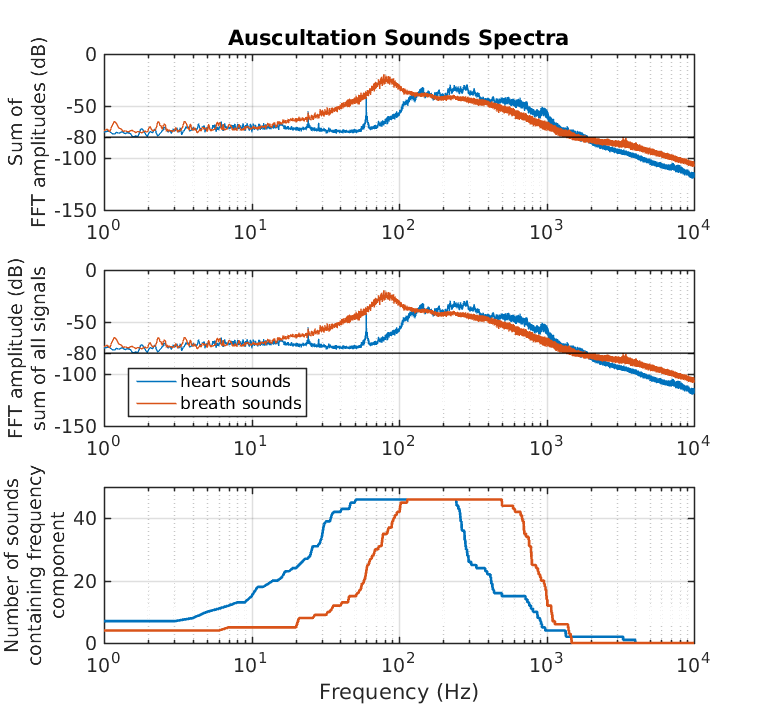
\includegraphics[width=120mm]{auscultation_spectra3.png}
	}
	\caption{Frequency spectra of auscultation sounds}
	\label{fig:ausc_spectra}
\end{figure}

\section{Sensor}
Why we chose microphone vs. laser mic, vs. cap sensor \\
How we coupled microphone to stethoscope \\
Microphone circuit

\section{Signal Amplification}
Instrumentation amplifier
Low pass filter
Amplifier

\section{Input Circuitry}
DC blocker to block out any DC ofset from amplification stage\\
1.6V summing circuit to allow maximum swing\\
clipping circuit to protect 0-3.3V range \\

\section{Signal Processing}
Why we needed and chose the dsPIC33FJ
Explain how code for dspic works

\section{Wireless Transmission}
Yudong

\section{Wired Transmission}
Yudong

\section{System Power}
Yudong